% Set title page for separate titlepage
\documentclass[titlepage]{article}

% Some standard math packages
\usepackage{amsmath}
\usepackage{amssymb}
\usepackage{amsfonts}
% Package for lists
\usepackage[shortlabels]{enumitem}
% Dashed lines
\usepackage{arydshln}
% Graphics
\usepackage{tikz}

\title{Bound Entanglement and Bound Information \\ - \\ BSc Project Plan}

\author{Luca Dolfi\\ Advisor: Stefan Wolf \\ Tutor: Arne Hansen}
\date{Spring 2018}

\begin{document}
\maketitle
\section*{Motivation}
One can show that there exists a correspondence between entanglement distillation in quantum mechanics and classical key agreement in information theory. In the same quantum-mechanical framework there are, furthermore, non-distillable, but entangled quantum states. So, considering the above analogy, does there exists some notion of bound information?

Following the intuition from the analogies of classical key agreement with entanglement distillation together with the features of bound entanglement one might hope to find characteristics/limitations of information-theoretic concepts.

\section*{Project Description}
Entanglement---a consequence of the linear structure of the mathematical
formalism of quantum mechanics---is one of the astounding aspects of
quantum mechanics and a valuable resource for a number of computational
tasks.
To measure entanglement one might consider the least number of maximally
entangled bipartite quantum states---so-called singlets---required to
prepare a density matrix $\rho$ by local operations and classical
communication.
Similarly one might measure entanglement by the maximal number of
singlets that can be obtained form $\rho$ by local operations and
classical communication.
These measures are not the same. Particularly, there exists weakly
entangled states---called bound-entangled---that require singlets for
their preparation while they, in turn, do not allow to distill any singlets.

There are analogies to classical key agreement, for instance,
entanglement distillation schemes based on protocols for classical key
agreement.
Together with an information-theoretic analogue for the entanglement
cost, the so-called \emph{information of formation} or \emph{key cost},
one can ask whether there exists an information-theoretic analogue to
bound entanglement.
Is there a tripartite probability distribution, corresponding to Alice
and Bob wanting to establish a key unknown to Eve, that has a non-zero
key cost, while not allowing to distill any secret key?

\section*{Goals}
The aim of this project is to build an understanding of bound
entanglement, the related measures of entanglement and their connections
to concepts of classical key agreement, as well as related
information-theoretic concepts, in order to approach this open question.

\pagebreak

\section*{Schedule}

Although the project is mainly a research investigation the future work can be divided in the following tasks and milestones \\
\begin{enumerate}[A)]
\item Project assessment
\item Concepts of QM
\item Concepts of information theory
\item Investigation into bound information / Final submission
\end{enumerate}
\centerline{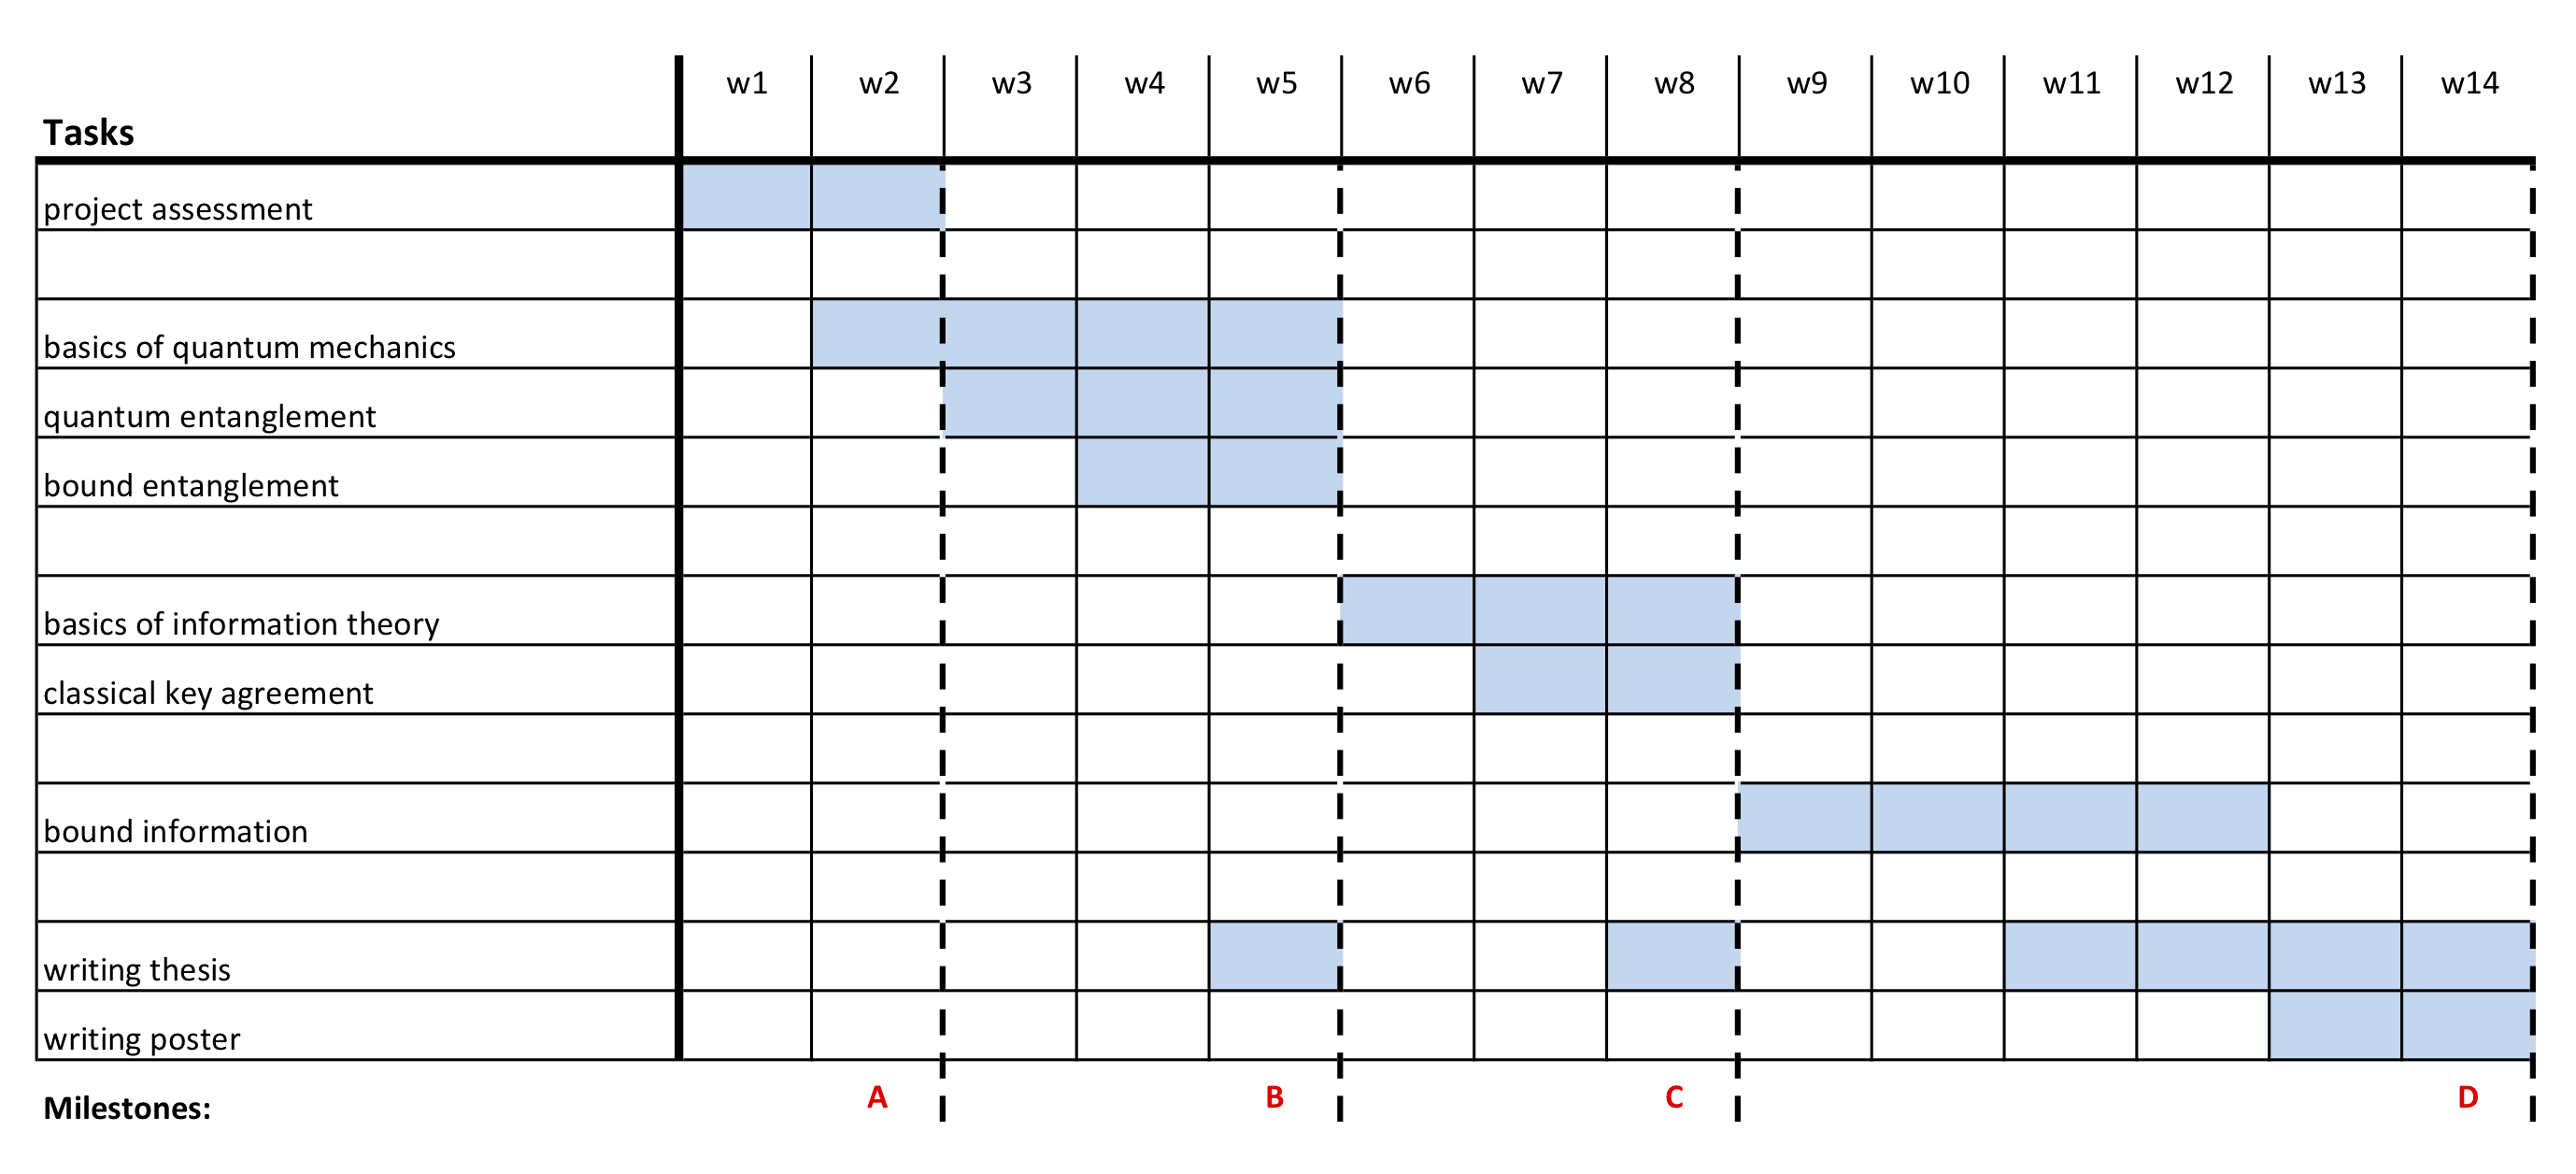
\includegraphics[scale=0.2, angle=-90]{planning2.png}}

\end{document}
